\documentclass[12pt]{article}    
\usepackage{ucs} 
\usepackage[utf8x]{inputenc}
\usepackage[russian]{babel}  
\usepackage{float}
\title{Лабораторная работа №4\\Маятник Обербека}
\author{Хафизов Фанис}
\usepackage[pdftex]{graphicx}

\begin{document}
	\begin{figure}
		\centering
		
\includegraphics[width=0.3\linewidth]{logo}
	\end{figure}
	\maketitle
	\newpage
	\section{Цель работы}
	Цель данной лабораторной работы состоит в экспериментальном изучении законов динамики вращательного движения твердого тела от распределения массы
	относительно неподвижной оси вращения. Момент инерции тела является мерой инертности тела при вращательном движении и аналогичен массе тела при
	его поступательном движении.
	\section{Схема установки}
	\begin{figure}[H]
		\centering
		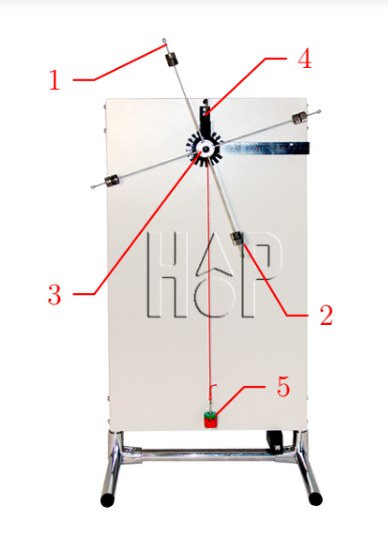
\includegraphics[scale=0.5]{scheme}
		\caption{Схема установки}
	\end{figure}
	Маятник Обербека (рис. 1) представляет собой крестовину (1), на вращающейся оси (3),
на шкив которой намотана нить с грузиком (5)
массой m0. На четырех взаимно перпендикулярных стержнях крестовины располагаются четыре подвижных груза (2) массой m каждый. Под действием силы тяжести груза (5)
нить разматывается с оси и вызывает вращательное движение крестовины. На оси крестовины располагается датчик (4) угловой скорости вращения маятника.	К приборам и принадлежностям 		относятся
также компьютер с необходимым программным обеспечением и 					соединительный кабель
для подключения датчика угловой скорости к
компьютеру.
	\section{Порядок действий}
	1)Соберем экспериментальную установку и разместим грузики на расттоянии $r_1$.\\
	2)Приведем маятник в движение и запустим измерения.\\
	3)Остановим измерения, когда маятник достигнет нижней точки.\\
	4)Внесем данные с графика в таблицу на участке, где зависимсть линейна.\\
	5)Найдем угловой ускорение как угловой коэффициент зависимости $\omega(t)$.\\
	6)Повторим пп. 1-5, установив грузики теперь на расстоянии $r_2$.\\
	\section{Таблицы данных и графики}
	\begin{table}[H]
		\centering
		\caption{Входные данные}
		\begin{tabular}{|l|l|l|l|l|}
			\hline
			m, г       & d, мм      & $m_0$, г    & $r_1$, мм & $r_2$, мм \\ \hline
			52$\pm$0,5 & 30$\pm$0,5 & 105$\pm$0,5 & 200$\pm$1 & 150$\pm$1 \\ \hline
		\end{tabular}
	\end{table}
	\begin{table}[H]
		\centering
		\caption{}
		\begin{tabular}{|l|l|l|l|l|l|}
			\hline
			i & $\varepsilon_{i1}$, с$^{-2}$ & $\varepsilon_{1}$, с$^{-2}$ & $\varepsilon_{i2}$, с$^{-2}$ & $\varepsilon_{2}$, с$^{-2}$ & $J_c$, кг$\cdot$м$^2$ \\ \hline
			1 & 1,45                       &                           & 2,31                       &                           &                       \\ \cline{1-2} \cline{4-4}
			2 & 1,41                       &                           & 2,29                       &                           &                       \\ \cline{1-2} \cline{4-4}
			3 & 1,43                       & 1,44                      & 2,31                       & 2,32                      & $1{,}253\cdot10^{-3}$  \\ \cline{1-2} \cline{4-4}
			4 & 1,45                       &                           & 2,34                       &                           &                       \\ \cline{1-2} \cline{4-4}
			5 & 1,45                       &                           & 2,34                       &                           &                       \\ \hline
		\end{tabular}
	\end{table}
	\begin{figure}[H]
		\centering
		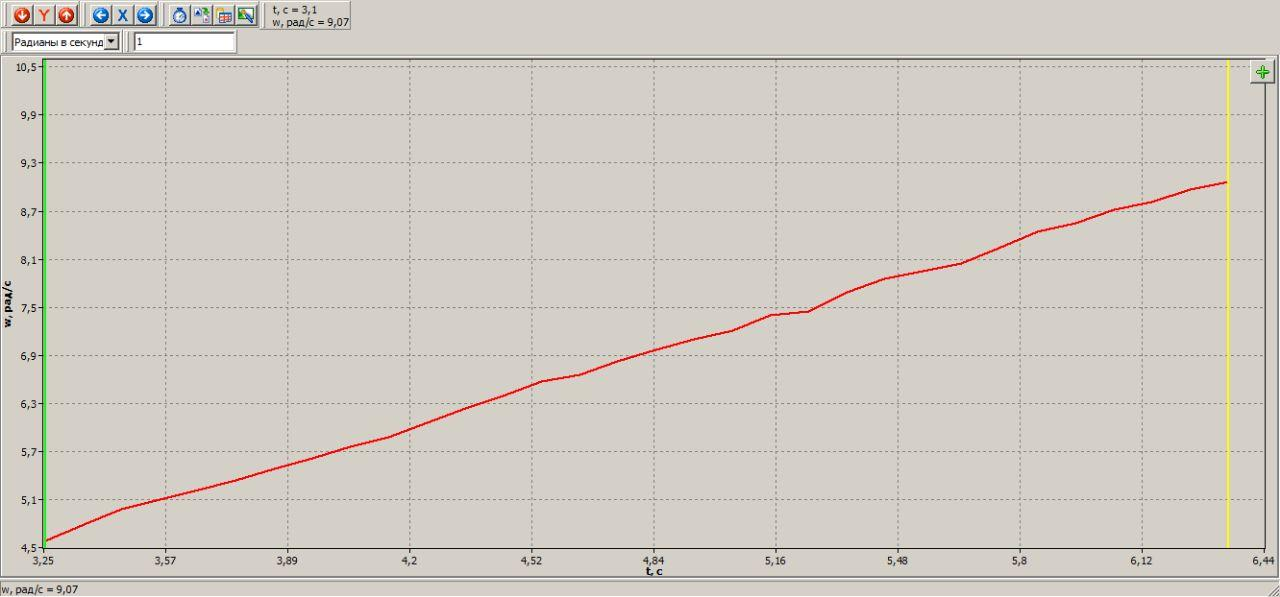
\includegraphics[scale=0.45]{graph1}
		\caption{График зависимости $\omega(t)$}
	\end{figure}
	\begin{figure}[H]
		\centering
		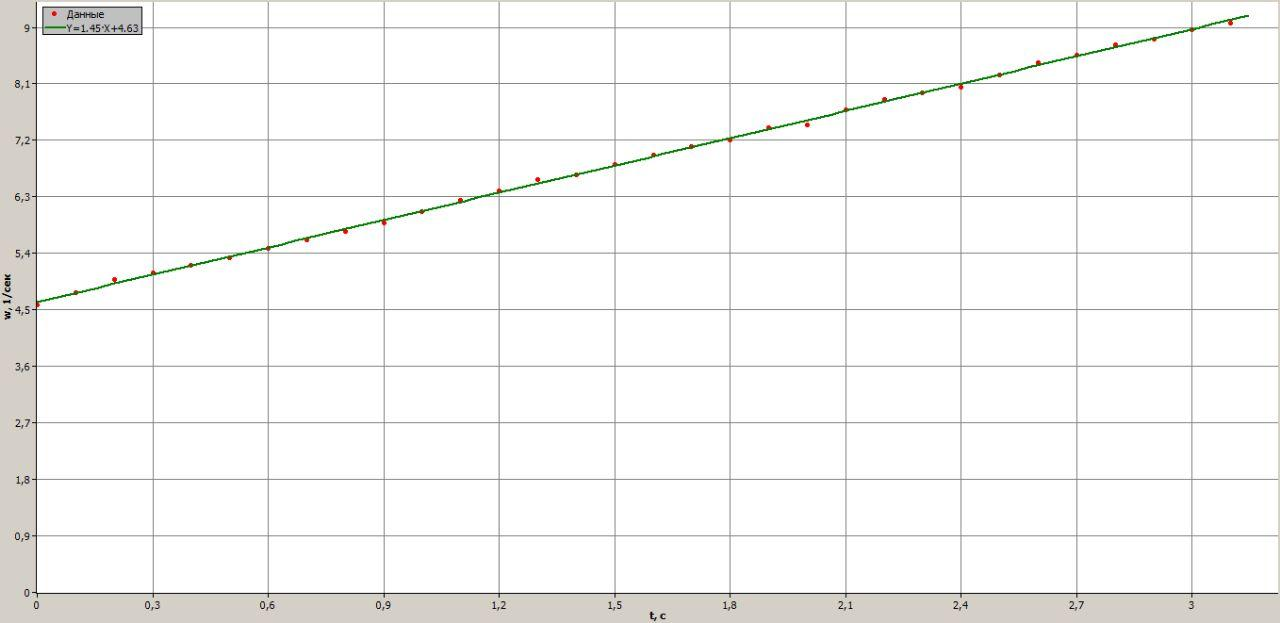
\includegraphics[scale=0.45]{graph2}
		\caption{График зависимости $\omega(t)$, аппроксимированный прямой}
	\end{figure}
	\section{Расчеты}
	$J_c=4m\frac{r_2^2\varepsilon_{2}-r_1^2\varepsilon_{1}}{\varepsilon_{1}-\varepsilon_{2}}-m_0\frac{d^2}{4}=4\cdot0{,}052\frac{0{,}15^2\cdot2{,}32-0{,}2^2\cdot1{,}44}{1{,}44-2{,}32}-0{,}105\frac{0{,}03^2}{4}=1{,}253\cdot10^{-3}$ кг$\cdot$м$^2$\\
	$\sigma_{\varepsilon1}=\sqrt{\frac{\sum\limits_{i=1}^5(\varepsilon_{1i}-\overline{\varepsilon}_{1})}{5}}=0{,}02$ c$^{-2}$\\
	$\sigma_{\varepsilon2}=\sqrt{\frac{\sum\limits_{i=1}^5(\varepsilon_{2i}-\overline{\varepsilon}_{2})}{5}}=0{,}02$ c$^{-2}$\\
	$\Delta\varepsilon_{1}=2\sigma_{\varepsilon1}=0{,}04$ c$^{-2}$\\
	$\Delta\varepsilon_{2}=2\sigma_{\varepsilon2}=0{,}04$ c$^{-2}$\\
	$\Delta J_c=(\frac{\Delta m}{m}+\frac{(\frac{2\Delta r_2}{r_2}+\frac{\Delta\varepsilon_{2}}{\varepsilon_{2}})r_2^2\varepsilon_{2}+(\frac{2\Delta r_1}{r_1}+\frac{\Delta\varepsilon_{1}}{\varepsilon_{1}})r_1^2\varepsilon_{1}}{r_2^2\varepsilon_{2}-r_1^2\varepsilon_{1}}+\frac{\Delta\varepsilon_{1}+\Delta\varepsilon_{2}}{\varepsilon_{1}-\varepsilon_{2}})4m\frac{r_2^2\varepsilon_{2}-r_1^2\varepsilon_{1}}{\varepsilon_{1}-\varepsilon_2}+(\frac{\Delta m_0}{m_0}+\frac{2\Delta d}{d})m_0\frac{d^2}{4}=0{,}981\cdot10^{-3}$ кг$\cdot$м$^2$\\
	$\delta J_c=\frac{\Delta J_c}{J_c}=0{,}78$\\
	\section{Результаты}
	$J_c=(1{,}253\pm0{,}981)$ кг$\cdot$м$^2$\\
	$\delta J_c=78\%$\\
	\section{Вывод}
	Сложно оценить, насколько близок результат к истине, но величина относительной погрешности очень велика и составляет 78\%. Это произошло, потому что в расчетной формуле 3 разности. Для увеличения точности можно было бы использовать другой метод измерения момента инерции. 
\end{document}